\documentclass[12pt,a4paper]{article}

% --- 核心宏包 ---
\usepackage[utf8]{inputenc}
\usepackage[T1]{fontenc}
\usepackage{ctex} % 中文支持 (如果使用 XeLaTeX，建议换成 ctex 宏包)
\usepackage{amsmath, amsfonts, amssymb}
\usepackage{geometry}
\geometry{left=2.5cm, right=2.5cm, top=3cm, bottom=3cm}

% --- 视觉与排版优化宏包 ---
\usepackage[table]{xcolor} % 颜色支持，带有表格填色功能
\usepackage{booktabs}      % 三线表美化
\usepackage{fancyhdr}      % 自定义页眉页脚
\usepackage[many]{tcolorbox} % 强大的带框/背景盒工具
\usepackage{enumitem}      % 列表间距调整
\usepackage{hyperref}      % 交叉引用与超链接
\usepackage{tikz}
\usetikzlibrary{positioning, arrows.meta} % 必须有 positioning
% --- 自定义颜色 (现代科技风) ---
\definecolor{macblue}{RGB}{0, 122, 255}    % 强调蓝
\definecolor{bglight}{RGB}{245, 245, 247}  % 极简浅灰背景
\definecolor{darkgray}{RGB}{51, 51, 51}
\definecolor{warningred}{RGB}{255, 59, 48} % 增加红色用于攻击/警告的强调
% --- 超链接设置 ---
\hypersetup{
    colorlinks=true,
    linkcolor=macblue,
    urlcolor=macblue
}

% --- 页眉页脚设置 ---
\pagestyle{fancy}
\fancyhf{}
\fancyhead[L]{\textcolor{macblue}{\textbf{Cryptography Notes}}}
\fancyhead[R]{\textbf{Data Encryption Standard (DES)}}
\fancyfoot[C]{\thepage}
\renewcommand{\headrulewidth}{0.8pt}
\renewcommand{\headrule}{\hbox to\headwidth{\color{macblue}\leaders\hrule height \headrulewidth\hfill}}

% --- 自定义高亮公式框 ---
\newtcolorbox{coreconcept}[1][]{
    colback=bglight,
    colframe=macblue,
    fonttitle=\bfseries\sffamily,
    title=#1,
    arc=3mm,
    boxrule=1.2pt,
    shadow={2mm}{-1.5mm}{0mm}{black!15},
    left=10pt, right=10pt, top=5pt, bottom=5pt
}
\newtcolorbox{warningbox}[1][]{
    colback=warningred!5,
    colframe=warningred,
    fonttitle=\bfseries\sffamily,
    title=#1,
    arc=3mm,
    boxrule=1.2pt,
    left=10pt, right=10pt, top=5pt, bottom=5pt
}

% --- 标题区域重塑 ---
\title{
    \vspace{-2cm}
    \color{macblue}\Huge\textbf{Data Encryption Standard (DES)}\\
    \vspace{0.5cm}
    \Large\textcolor{darkgray}{密码学核心算法学习笔记}
    \vspace{0.5cm}
}
\author{\textbf{Infinite}}
\date{\today}

\begin{document}

\maketitle
\thispagestyle{fancy} % 首页也显示漂亮页眉

\section{DES 算法架构概览}
DES 是一种经典的对称密钥分组密码（Block Cipher），它的设计奠定了现代密码学的基础。核心参数一览：
\begin{itemize}[itemsep=4pt, parsep=0pt]
    \item \textbf{明文分组长度：} 64 bit
    \item \textbf{有效密钥长度：} 56 bit \textit{（注：原始 64 bit 中有 8 bit 为奇偶校验位）}
    \item \textbf{迭代轮数：} 16 轮
    \item \textbf{核心结构：} Feistel 网络
\end{itemize}

\section{Feistel 网络数学模型}
DES 的每一轮迭代都遵循 Feistel 结构。其最大的优势在于\textbf{加密和解密可以使用完全相同的硬件/算法逻辑}，只需将子密钥逆序使用即可。

\begin{coreconcept}[第 $i$ 轮迭代公式]
设输入为 $L_{i-1}$ 和 $R_{i-1}$，第 $i$ 轮的子密钥为 $K_i$，则输出计算如下：
\begin{equation}
\begin{cases}
    L_i = R_{i-1} \\
    R_i = L_{i-1} \oplus F(R_{i-1}, K_i)
\end{cases}
\end{equation}
\textit{* 其中 $\oplus$ 表示按位异或运算，F 为非线性轮函数。}
\end{coreconcept}

\section{轮函数 $F$ 的内部剥析}
轮函数是 DES 安全性的核心，它负责引入混淆（Confusion）和扩散（Diffusion）。具体分为四个流水线步骤：
\begin{enumerate}[label=\textbf{Step \arabic*.}, itemsep=5pt]
    \item \textbf{扩展置换 (E-Box)：} 将 32 bit 的右半部分扩展为 48 bit。
    \item \textbf{密钥混合：} 与 48 bit 的本轮子密钥 $K_i$ 进行异或。
    \item \textbf{S-盒代换 (S-Box)：} \textcolor{red}{\textbf{DES 中唯一的非线性操作}}。将 48 bit 压缩回 32 bit。
    \item \textbf{P-盒置换 (P-Box)：} 将 32 bit 再次打乱位置，为下一轮做准备。
\end{enumerate}

\section{非线性核心：S-Box 示例}
DES 共包含 8 个 S-Box，每个 S-Box 接收 6 bit 输入，输出 4 bit。以下是 $S_1$ 盒的置换表设计：

\begin{table}[h]
    \centering
    \renewcommand{\arraystretch}{1.3} % 增加行高，更透气
    \rowcolors{2}{white}{bglight} % 斑马线：白灰交替
    \begin{tabular}{c|cccccccccccccccc}
        \toprule
        \rowcolor{macblue!10} % 表头浅蓝色背景
        \textbf{Row \textbackslash{} Col} & \textbf{0} & \textbf{1} & \textbf{2} & \textbf{3} & \textbf{4} & \textbf{5} & \textbf{6} & \textbf{7} & \textbf{8} & \textbf{9} & \textbf{10} & \textbf{11} & \textbf{12} & \textbf{13} & \textbf{14} & \textbf{15} \\
        \midrule
        \textbf{0} & 14 & 4 & 13 & 1 & 2 & 15 & 11 & 8 & 3 & 10 & 6 & 12 & 5 & 9 & 0 & 7 \\
        \textbf{1} & 0 & 15 & 7 & 4 & 14 & 2 & 13 & 1 & 10 & 6 & 12 & 11 & 9 & 5 & 3 & 8 \\
        \textbf{2} & 4 & 1 & 14 & 8 & 13 & 6 & 2 & 11 & 15 & 12 & 9 & 7 & 3 & 10 & 5 & 0 \\
        \textbf{3} & 15 & 12 & 8 & 2 & 4 & 9 & 1 & 7 & 5 & 11 & 3 & 14 & 10 & 0 & 6 & 13 \\
        \bottomrule
    \end{tabular}
    \caption{$S_1$ 盒替换矩阵 (6-bit to 4-bit)}
\end{table}

\section{查表攻击 (Lookup Table Attack)}
查表攻击是一种极其经典且直观的破解手段，常用于破解哈希值（如用户登录密码）或攻击密钥空间较小的加密算法。

\begin{coreconcept}[核心思想：空间换时间 (Time-Memory Trade-off)]
在传统的暴力破解（Brute Force）中，攻击者需要每次临时计算哈希，消耗大量 CPU/GPU 时间。查表攻击通过\textbf{预计算（Precomputation）}，提前将所有可能的“明文-哈希值”对计算并存储在数据库中。攻击时只需进行检索（Lookup），将漫长的“计算时间”压缩成了极短的“查询时间”。
\end{coreconcept}

\subsection{工作原理}
\begin{enumerate}[label=\textbf{\arabic*.}, itemsep=5pt]
    \item \textbf{预计算阶段：} 遍历字典（如常用密码组合），计算出对应的哈希值。例如，计算 $MD5(\text{infinite}) = \text{0db9bd68...}$。
    \item \textbf{构建数据字典：} 将键值对存入数据库，并以\textbf{哈希值}建立索引，以便反向查询。
    \item \textbf{攻击阶段：} 拿到泄露的哈希值后，直接在表中搜索，匹配成功即刻获得明文。
\end{enumerate}

\begin{warningbox}[查表攻击的致命弱点：存储爆炸]
如果密码是 8 位以上包含大小写及特殊字符的组合，所有可能结果的哈希表体积将达到 PB 甚至 EB 级别，超出普通硬盘的存储极限。
\end{warningbox}

\section{进阶形态：彩虹表 (Rainbow Table)}
为了突破存储瓶颈，查表攻击进化出了\textbf{彩虹表}。它在“计算时间”和“存储空间”之间找到了完美的平衡点，不再存储所有完整的键值对，而是只存储计算链条的\textbf{起点}和\textbf{终点}。

\subsection{彩虹链条构造}
彩虹表依靠两个核心函数交替运行来构建长长的链条：
\begin{itemize}
    \item \textbf{哈希函数 $H$ (Hash)：} 将明文单向映射为哈希值。
    \item \textbf{衰减函数 $R$ (Reduction)：} 将哈希值截断或转换为一个“伪明文”。\textit{（注：$R$ 绝不是 $H$ 的逆运算，它只负责生成下一个可以被哈希的合法输入）。}
\end{itemize}

\vspace{0.5cm}
% --- TikZ 绘制彩虹表链条图 ---
\begin{center}
\begin{tikzpicture}[node distance=2.5cm, auto, thick, >=stealth]
    % Nodes
    \node (p1) [draw, rounded corners, fill=macblue!10, text centered, inner sep=5pt] {明文 $P_1$};
    \node (h1) [right of=p1, draw, rounded corners, fill=gray!10, text centered, inner sep=5pt] {哈希 $H_1$};
    \node (p2) [right of=h1, draw, rounded corners, fill=macblue!10, text centered, inner sep=5pt] {明文 $P_2$};
    \node (h2) [right of=p2, draw, rounded corners, fill=gray!10, text centered, inner sep=5pt] {哈希 $H_2$};
    \node (dots) [right of=h2, xshift=-0.8cm] {$\cdots$};
    \node (pn) [right of=dots, xshift=-0.8cm, draw, rounded corners, fill=macblue!10, text centered, inner sep=5pt] {明文 $P_k$};
    \node (hn) [right of=pn, draw, rounded corners, fill=gray!10, text centered, inner sep=5pt] {哈希 $H_k$};

    % Arrows
    \draw[->, macblue] (p1) -- node[above] {$H$} (h1);
    \draw[->, warningred] (h1) -- node[above] {$R_1$} (p2);
    \draw[->, macblue] (p2) -- node[above] {$H$} (h2);
    \draw[->, warningred] (h2) -- node[above] {$R_2$} (dots);
    \draw[->, macblue] (pn) -- node[above] {$H$} (hn);
\end{tikzpicture}
\end{center}
\vspace{0.2cm}

生成数万步的链条后，数据库中\textbf{仅保存链条的首尾}：$(P_1, H_k)$。这使得存储空间缩小了成千上万倍。破解时，用目标哈希值不断交替进行 $R$ 和 $H$ 运算，看是否能撞上表中的终点 $H_k$，如果撞上，就能顺藤摸瓜找回起点的明文。

\section{终极防御：加盐 (Salting)}
防御预计算攻击（包括彩虹表）最简单、最有效的方法就是\textbf{加盐（Salt）}。

\begin{coreconcept}[加盐机制]
在将用户密码（如 \texttt{infinite}）进行哈希处理前，系统随机生成一段字符串（如 \texttt{\&x9q}）附加在密码中，即 $Hash(\texttt{infinite} + \texttt{\&x9q})$。这个随机字符串就是“盐”，它会与哈希值一并明文存入数据库。
\end{coreconcept}

\textbf{防御原理：} 由于每个用户的“盐”都是随机且不同的，攻击者如果想用查表攻击，就必须为\textbf{每一个不同的盐}单独生成一张极其巨大的彩虹表。这在计算能力和存储空间上都是绝对不可能完成的任务，从而彻底废掉了攻击者预计算的优势。
\section{针对 DES 的查表攻击实战}
在分析 DES 算法的安全性时，查表攻击通常建立在\textbf{已知明文攻击 (KPA, Known Plaintext Attack)} 的假设前提下。假设攻击者已经截获了一对匹配的明文 $P_0$ 和密文 $C_0$，其目标是逆推出加密使用的 56-bit 密钥 $K$。

\subsection{朴素查表法与存储爆炸}
在朴素的查表攻击中，攻击者会针对已知的明文 $P_0$，使用全部可能的密钥进行预计算。

\begin{enumerate}[label=\textbf{Step \arabic*.}, itemsep=5pt]
    \item \textbf{预计算字典：} 遍历 DES 的 $2^{56}$ 个可能密钥。对于每一个密钥 $K_i$，计算 $C_i = E_{K_i}(P_0)$。
    \item \textbf{建表排序：} 将所有的 $(C_i, K_i)$ 键值对存入数据库，并按照密文 $C_i$ 进行排序，建立索引。
    \item \textbf{极速破解：} 当拿到目标密文 $C_0$ 时，直接在表中进行二分查找。只需极短的时间，就能直接查出对应的密钥 $K$。
\end{enumerate}

\begin{warningbox}[可行性灾难：计算一下 DES 朴素查表的体积]
虽然 DES 的 $2^{56}$（约 $7.2 \times 10^{16}$）密钥空间在今天的算力下可以被穷举，但要把它们全部存下来却是个噩梦：
\begin{itemize}
    \item 每个条目包含密文（64 bit = 8 Byte）和密钥（56 bit = 7 Byte），共 15 Byte。
    \item 总存储量需求：$15 \times 2^{56} \text{ Bytes} \approx 1.08 \times 10^{18} \text{ Bytes} \approx \textbf{1.08 Exabytes (EB)}$。
\end{itemize}
建立一个 1 EB 的高速查询数据库在工程上是不现实的。因此，纯粹的朴素查表法对 DES 无效。
\end{warningbox}

\subsection{破局：赫尔曼时间-空间折中 (Hellman's TMTO)}
为了解决 DES 查表攻击的存储瓶颈，Martin Hellman 在 1980 年提出了著名的\textbf{时间-空间折中理论 (Time-Memory Trade-Off)}。这也是现代彩虹表技术的直接理论前身。

Hellman 提出，不必把 $2^{56}$ 个状态全部存下来，而是通过构造链条来压缩数据：
\begin{coreconcept}[Hellman 针对 DES 的链条构造]
\begin{itemize}
    \item \textbf{加密函数 (相当于 H)：} $C = E_K(P_0)$。以固定明文 $P_0$ 对密钥 $K$ 进行加密，输出 64-bit 密文。
    \item \textbf{约化函数(Reduction function) $R$：} 将 64-bit 的密文映射回 56-bit 的密钥空间。简单做法是直接丢弃 8 个 bit，使其成为下一个要测试的“伪密钥”。
\end{itemize}
通过交替执行 $E$ 和 $R$，生成长度为 $t$ 的长链：
$$ K_1 \xrightarrow{E_{P_0}} C_1 \xrightarrow{R} K_2 \xrightarrow{E_{P_0}} C_2 \xrightarrow{R} \cdots \xrightarrow{R} K_t $$
\end{coreconcept}

最终，黑客的硬盘里\textbf{只保存链条的起点 $K_1$ 和终点 $K_t$}。
通过这种折中方案，Hellman 证明了在已知部分明文的情况下，攻击者可以牺牲部分在线计算时间（用于在链条中游走查找），将原本需要 1 EB 的存储空间压缩到\textbf{几百 GB 甚至更小}的级别，从而让针对 DES 的查表攻击从“理论”变成了“现实威胁”。
\begin{itemize}
    \item 预计算阶段：构造 $s$ 个预计算表 $\mathbb{T}_\alpha$ ($\alpha = 1, \cdots, s$)，每个预计算表的构造方式如下 (如图 4.7 所示).
\end{itemize}

% --- 图 4.7 绘制 ---
\begin{figure}[htbp]
    \centering
    \setlength{\tabcolsep}{2pt}
    \begin{tabular}{|c|ccccccc|c|}
        \cline{1-1} \cline{9-9}
        $k_{1,0}$ & $\xrightarrow{g}$ & $k_{1,1}$ & $\xrightarrow{g}$ & $k_{1,2}$ & $\xrightarrow{g}$ & $\cdots$ & $\xrightarrow{g}$ & $k_{1,t}$ \\
        $k_{2,0}$ & $\xrightarrow{g}$ & $k_{2,1}$ & $\xrightarrow{g}$ & $k_{2,2}$ & $\xrightarrow{g}$ & $\cdots$ & $\xrightarrow{g}$ & $k_{2,t}$ \\
        $\vdots$ & & \vdots & & \vdots & & $\ddots$ & & $\vdots$ \\
        $k_{q,0}$ & $\xrightarrow{g}$ & $k_{q,1}$ & $\xrightarrow{g}$ & $k_{q,2}$ & $\xrightarrow{g}$ & $\cdots$ & $\xrightarrow{g}$ & $k_{q,t}$ \\
        \cline{1-1} \cline{9-9}
    \end{tabular}
    \caption{时间-存储权衡攻击的预计算表 $\mathbb{T}_\alpha$ 的构造}
\end{figure}

\begin{enumerate}
    \item 随机选择 $q$ 个长度为 $l$-bit 的数据 $k_{1,0}, k_{2,0}, \cdots, k_{q,0}$.
    \item 任意取定一个明文 $m^*$，对 $i = 1, \cdots, q$, $j = 1, \cdots, t$，计算
    $$k_{i,j} = g(k_{i,j-1}) = R_\alpha(Enc_{k_{i,j-1}}(m^*)),$$
    其中，$g$ 为链接函数，由函数 $R$ 与加密算法 $Enc$ 构成，函数 $R$ 为 $\{0, 1\}^n \to \{0, 1\}^l$ 的函数，主要用于将 $n$-bit 的密文转化为 $l$-bit 的密钥 (具体可通过第 6 章介绍的杂凑函数或简单截短来实现)，因此，函数 $R$ 被称为约化函数. 不同的 $\alpha$，对应不同的函数 $R$，记为 $R_\alpha$.

    此步骤借助明文 $m^*$ 的加密及约化函数在密钥之间形成链条. 可见，只要知道起点 $k_{i,0}$ ($i = 1, \cdots, q$)，就可以计算出同一条链上的所有密钥.
    
    \item 存储每条链的起点 $k_{i,0}$ 和终点 $k_{i,t}$\footnotemark[1].
\end{enumerate}

\footnotetext[1]{存储时以 $k_{i,t}$ 为索引.}

\begin{itemize}
    \item 在线阶段：选择明文 $m^*$，获得对应的密文 $c^*$. 对 $\alpha = 1, \cdots, s$，即每个预计算表 $\mathbb{T}_\alpha$，
\end{itemize}

\begin{enumerate}
    \item 计算 $c_1 = R_\alpha(c^*)$.
    \item 对 $j = 1, \cdots, t$，比较 $c_j$ 与每条链的终点 $k_{i,t}$ ($i = 1, \cdots, q$)：
    
    若存在 $i$，满足 $c_j = k_{i,t}$，则从 $k_{i,0}$ 出发计算出 $k_{i,t-j}$. 代入 $c^* = Enc_{k_{i,t-j}}(m^*)$ 进行验证. 若成立，将 $k_{i,t-j}$ 作为正确密钥的候选值.
    
    否则，计算 $c_{j+1} = g(c_j)$，继续与终点进行比较.
    \item 若可能正确的密钥个数多于 1 个，再结合已知明密文对，做进一步筛选.
\end{enumerate}

下面，对以上正确密钥的判定依据给出简要分析. 如图 4.8 所示，

% --- 图 4.8 绘制 ---
\begin{figure}[htbp]
    \centering
    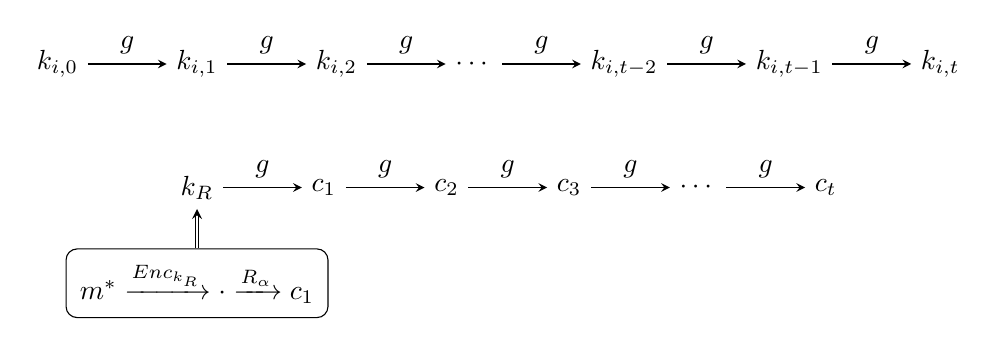
\begin{tikzpicture}[node distance=1.2cm and 1cm, auto, >=stealth]
        % 第一行链条
        \node (k0) {$k_{i,0}$};
        \node (k1) [right=of k0] {$k_{i,1}$};
        \node (k2) [right=of k1] {$k_{i,2}$};
        \node (dots1) [right=of k2] {$\cdots$};
        \node (ktm2) [right=of dots1] {$k_{i,t-2}$};
        \node (ktm1) [right=of ktm2] {$k_{i,t-1}$};
        \node (kt) [right=of ktm1] {$k_{i,t}$};

        \draw[->] (k0) -- node[above] {$g$} (k1);
        \draw[->] (k1) -- node[above] {$g$} (k2);
        \draw[->] (k2) -- node[above] {$g$} (dots1);
        \draw[->] (dots1) -- node[above] {$g$} (ktm2);
        \draw[->] (ktm2) -- node[above] {$g$} (ktm1);
        \draw[->] (ktm1) -- node[above] {$g$} (kt);

        % 第二行链条
        \node (kr) [below=1cm of k1] {$k_R$};
        \node (c1) [right=of kr] {$c_1$};
        \node (c2) [right=of c1] {$c_2$};
        \node (c3) [right=of c2] {$c_3$};
        \node (dots2) [right=of c3] {$\cdots$};
        \node (ct) [right=of dots2] {$c_t$};

        \draw[->] (kr) -- node[above] {$g$} (c1);
        \draw[->] (c1) -- node[above] {$g$} (c2);
        \draw[->] (c2) -- node[above] {$g$} (c3);
        \draw[->] (c3) -- node[above] {$g$} (dots2);
        \draw[->] (dots2) -- node[above] {$g$} (ct);

        % 左下角的明文加密框
        \node[draw, rounded corners, below=0.5cm of kr, inner sep=5pt] (box) {
            $m^* \xrightarrow{Enc_{k_R}} \cdot \xrightarrow{R_\alpha} c_1$
        };
        \draw[->, double] (box.north) -- (kr.south);

    \end{tikzpicture}
    \caption{时间-存储权衡攻击在线阶段示例}
\end{figure}

$$c_1 = R_\alpha(c^*) = R_\alpha(Enc_{k_R}(m^*)) = g(k_R).$$
即若以正确密钥 $k_R$ 为起点，构造密钥链条，则 $c_j$ ($j = 1, \cdots, t$) 组成链条上的点.

若存在 $c_j = k_{i,t}$，例如，$c_2 = k_{i,t}$，则有
$$g(g(k_R)) = g(k_{i,t-1}) = g(g(k_{i,t-2})).$$
函数 $g \cdot g$ 的输出 $c_2$ 和 $k_{i,t}$ 相等，很可能是由输入相等导致的. 即若 $k_{i,t-2}$ 是正确...

时间复杂度\(T=O(qts)+O(ts)\),空间复杂度\(M = O(qs)\)

需要保证我们中间的连接点中含有密钥，所以这个表其实还是要尽量覆盖整个密钥空间，但是由于我们只存了起点和终点，所以极大地缩小了存储的空间

也就是\(qts \approx 2^l\)


\subsection{防范与历史终结}
Hellman 提出 TMTO 的初衷就是为了警告世人 DES 的 56-bit 密钥太短。防御这种高级查表攻击的最直接方式就是\textbf{增大密钥空间}（例如升级到 3DES 甚至 AES），当底层空间达到 $2^{128}$ 时，无论是计算量还是存储量，TMTO 链条都无法再被构建出来。

\subsection{差分攻击}
不随机现象产生了一个区分器
\[
Pr(c\oplus c' = m \oplus m') = 1
\]
3轮DES的差分传播
选择一对明文\((L_0,R_0),(L_0,R'_0)\)满足
\[
\Delta L_0 = L_0 \oplus L'_0 = 2 
\]
\[
\Delta R_0 = R_0 \oplus R'_0 = 0 
\]
经过一轮之后
\[
\Delta L_1 = L_1 \oplus L'_1 = R_0 \oplus R'_0 = 0 
\]
\[
\Delta R_1 = R_1 \oplus R'_1 = (L_0 \oplus f(K_0,R_0)) \oplus (L'_0 \oplus f(K_0,R'_0)) = 2
\]
第二轮
\[
\Delta L_2 = L_2 \oplus L'_2 = R_1 \oplus R'_1 = 2
\]
\[
\Delta R_2 = R_2 \oplus R'_2 = (L_1 \oplus f(K_1,R_1)) \oplus (L'_1 \oplus f(K_1,R'_1)) = \alpha
\]
第三轮我们不交换
\[
L_3 = L_2 \oplus f(K_2,R_2)
\]
\[
R_3 = R_2
\]
于是
\[
\Delta L_3 = (L_2 \oplus f(K_2,R_2)) \oplus (L'_2 \oplus f(K_2,R'_2))
\]
\[
\Delta R_3 = 0
\]
\section{线性分析}
如果密码算法只有线性运算，那很容易找到一个线性关系，例如矩阵等，是不安全的

所以必须引入非线性部件，例如S盒

考虑这个加密
\[
c = S(m\oplus k_0) \oplus k_1
\]

我们用线性掩码来刻画线性组合
\[
\vec{\alpha} \cdot \vec{v} =\alpha_0 v_0 \oplus \alpha_1 v_1 \oplus \cdots \oplus \alpha_{n-1} v_{n-1}
\]
表示将v中对应于a中非零位置的元素进行异或
\subsection{S盒的线性近似}
假设输入为X，输出为Y
则\(\alpha \cdot X \oplus \beta \cdot Y\)为S盒的一个线性近似式子

然后我们去考虑\(Pr(\alpha \cdot X \oplus \beta \cdot Y = 0)\),也就是\(Pr(\alpha \cdot X = \beta \cdot Y)\)

这个事件是否是一个随机事件？如果这个概率与随机置换不同，那么就可以作为一个区分器

我们去考虑随机置换成立的概率

他相当于一些随机比特的异或
\[
r_1 \oplus r_2 \oplus \cdots \oplus r_k = 0
\]
由于随机性，这个结果要么是0，要么是1，概率应该是0.5

那么我们可以用\(|Pr(\alpha \cdot X \oplus \beta \cdot Y = 0) - 0.5|\)来衡量这个线性近似的好坏

记为\(\epsilon = Pr(\alpha \cdot X \oplus \beta \cdot Y = 0) - 0.5\),\(|\epsilon|\)越大，说明这个线性近似越有效

这个线性表达式的目的，就是把左边变成明文和密文的线性组合，右边变成密钥的线性组合，从而消除掉中间变量

鉴于前面的例子，我们可以得到一个线性表达式
\[
\alpha \cdot m \oplus \beta \cdot c = (\alpha \cdot k_0 \oplus \beta \cdot k_1)
\]

假设这个概率以p的概率成立，然后我们得到N个明文密文对，那么这个线性表达式成立的次数应该是\(pN\)

总结成算法
\begin{enumerate}
    \item 初始化两个计数器\(T_0=0,T_1=0\)
    \item 计算\(b = \alpha \cdot m \oplus \beta \cdot c\),如果\(b=0\),则\(T_0 = T_0 + 1\),否则\(T_1 = T_1 + 1\)
    \item 如果\(T_0 > \frac{N}{2}\),当\(p>\frac{1}{2}\)时，猜测\(\alpha \cdot k_0 \oplus \beta \cdot k_1 = 0\),否则猜测\(\alpha \cdot k_0 \oplus \beta \cdot k_1 = 1\)
\end{enumerate}

得到一个表达式，就可以恢复一个比特的密钥信息，
\end{document}